%\newpage
\section{Nonlinear classifiable sets}
In the section, we will extend the linearly separable sets to the nonlinear case. 
A natural extension is like what the kernel method does in SVM for binary case. We will introduce the so-called 
feature mapping.

%Thus, we have the following natural extension for linearly separable by using feature mapping and original definition of linearly separable.

\begin{definition}[nonlinearly separable sets]
	These data sets $A_1, A_2, \cdots, A_k \subset \mathbb{R}^d$ are called nonlinearly separable, if there exist
	a feature space $\mathbb{R}^{\tilde d}$ and a smooth (if it has derivatives of all orders) feature mapping 
	\begin{equation}\label{key}
	\varphi: \mathbb{R}^d \mapsto \mathbb{R}^{\tilde d}
	\end{equation}
	such that
	\begin{equation}\label{key}
	\tilde A_i := \varphi(A_i) = \{ \tilde x ~|~ \tilde x = \varphi(x), x \in A_i \}, \quad i = 1, 2, \dots, k,
	\end{equation}
	are linearly separable.
\end{definition}

\begin{remark}$ $\\
	\begin{enumerate}
		\item This definition is  consistent with the definition of linearly separable as we can just take $\tilde d = d$ and $\varphi = {\rm id}$ if $A_1, A_2, \cdots, A_k$ are already linearly separable.
		\item The kernel method in SVM is mainly based on this idea for binary case (k=2) where they use kernel functions to approximate $\varphi(x)$.
		\item Most commonly used deep learning models are related to softmax mappings which means we can interpret these deep learning models as the approximation for feature mapping $\varphi$.
	\end{enumerate}	
\end{remark}


\begin{theorem}
	$A_1, A_2, \cdots, A_k \subset \mathbb{R}^d$ are nonlinearly separable  is equivalent to that there  
	 exists a smooth classification function 
	\begin{equation}\label{key}
	\psi: \mathbb{R}^d \mapsto \mathbb{R}^{k}
	\end{equation}
	such that for all $1\leq i \leq k$ and $ j \neq i$
	\begin{equation}\label{key}
	\psi_i (x) > \psi_j (x), \quad \forall x \in A_i.
	\end{equation}
\end{theorem}

\begin{proof}
	On the one hand, it is easy to see that if $A_1, A_2, \cdots, A_k \subset \mathbb{R}^d$ are nonlinearly separable, we can take 
	\begin{equation}\label{key}
	\psi(x) = \bm p(\varphi(x); \theta),
	\end{equation}	
	where $\bm p(\varphi(x); \theta)$ is the softmax function for linearly separable sets $\varphi(A_i)$ for $i=1,2,\cdots,k$.
	
	On the other hand, let assume that $\psi$ is the smooth classification functions for $A_1, A_2, \cdots, A_k \subset \mathbb{R}^d$. 
	We can take $\varphi(x) = \psi(x)$ and then
	\begin{equation}\label{key}
	\varphi(A_1), \varphi(A_2), \cdots, \varphi(A_k) \subset \mathbb{R}^k \quad ( \tilde d = k),
	\end{equation}
	will be linearly separable. Recall the definition of softmax mapping in Definition \ref{softmax}, if we take $\theta = (I, 0)$ in softmax mapping $\bm p(x;\theta)$, 
	then the monotonicity of $e^x$ shows that for all $i = 1:k$ and $ j \neq i$
	\begin{equation}\label{key}
	\bm p_i ( \varphi(x);\theta) = \frac{e^{\psi_i(x)}}{\sum_{i=1}^k e^{\psi_i(x)}} > \frac{e^{\psi_j(x)}}{\sum_{i=1}^k e^{\psi_i(x)}} = \bm p_j ( \varphi(x);\theta) , \quad \forall x \in A_i.
	\end{equation}
	
\end{proof}


Similar to linearly separable sets, we have the next lemma for $k=2$.
\begin{lemma}$A_1$ and $A_2 \subset \mathbb{R}^d$ are nonlinearly separable  is equivalent that there  
	exists a function $\varphi: \mathbb{R}^d \mapsto \mathbb{R}$ such that
	\begin{equation}\label{NonlinearBinary}
	\varphi(x) > 0 \quad \forall x \in A_1 \quad \text{and} \quad 	\varphi(x) < 0 \quad \forall x \in A_2.
	\end{equation}
\end{lemma}

\begin{proof}
On the one hand, based the equivalence of nonlinearly separable sets, there exists $\psi_1(x)$ and $\psi_2(x)$ such that 
for all $i = 1:2$ and $ j \neq i$
\begin{equation}\label{key}
\psi_i (x) > \psi_j (x), \quad \forall x \in A_i.
\end{equation}
Then, we can just take 
\begin{equation}\label{key}
\varphi(x) = \psi_1 (x) - \psi_2 (x).
\end{equation}

On the other hand, if there exist $\varphi(x)$ satisfies (\ref{NonlinearBinary}), then we can construct $\psi_1(x)$ and $\psi_2(x)$ as
\begin{equation}\label{key}
\psi_1(x) =  \frac{1}{2}\varphi(x) \quad \text{and}\quad 
\psi_2(x) = -\frac{1}{2}\varphi(x).
\end{equation}
\end{proof}


%\begin{definition}[nonlinearly separable]
%	These data sets $A_1, A_2, \cdots, A_k \subset \mathbb{R}^d$ are called nonlinearly separable, if there exist
%	a infinitely differentiable classification function 
%	\begin{equation}\label{key}
%	\psi: \mathbb{R}^d \mapsto \mathbb{R}^{k}
%	\end{equation}
%	such that for all $i = 1:k$ and $ j \neq i$
%	\begin{equation}\label{key}
%	\psi_i (x) > \psi_j (x), \quad \forall x \in A_i.
%	\end{equation}
%\end{definition}

\begin{remark}
%This definition is consistent with the original definition of linearly separable. 
%If $A_1, A_2, \cdots, A_k \subset \mathbb{R}^d$ are linearly separable, then there exists a $\theta$
%and softmax mapping $\bm p(x; \theta)$ such that for $i = 1:k$ and $ j \neq i$
%\begin{equation}\label{key}
%\bm p_i (x;\theta) > \bm p_j (x;\theta), \quad \forall x \in A_i.
%\end{equation}
%Thus, $A_1, A_2, \cdots, A_k$ are also nonlinearly separable as we can take $\psi(x) = \bm p(x;\theta)$.
Here the only assumption is that for all $i = 1:k$ and $ j \neq i$, we have $\psi_i (x) > \psi_j (x)$, $\forall x \in A_i$ for nonlinearly separable. We do not assume that $\psi_i (x) \ge 0$ or $\displaystyle\sum_{i=1}^k \psi_i (x) = 1$, which means that 
$$\psi(x) = \begin{pmatrix}
\psi_1 (x), &\psi_2 (x), &\cdots, &\psi_k (x)
\end{pmatrix}^T$$ 
is not a discrete probability distribution over all k classes. 
\end{remark}


The previous theorem shows that the softmax function is not so crucial in nonlinearly separable case. Combined with deep learning models, we have the 
following understanding about what deep learning models.
\begin{enumerate}
	\item If  the classification model is followed with a softmax, then it is approximating the feature mapping $\varphi: \mathbb{R}^d \mapsto \mathbb{R}^{\tilde d}$.
	\item If the classification model dose not followed by a softmax, then it is approximating $\psi: \mathbb{R}^d \mapsto \mathbb{R}^{k}$ directly.
\end{enumerate}
 
 
 \begin{example}
 	Consider $k=2$ and 
	$$
	A_1 \subset \{ (x_1, x_2) | x_1^2 + x_2^2 < 1\}, \quad A_2 \subset  \{(x_1, x_2) | x_1^2 + x_2^2 > 1\},
	$$
	then we have the following nonlinear
 	 feature mapping:
 	 \begin{equation*}
 	 \adjustbox{valign=c}{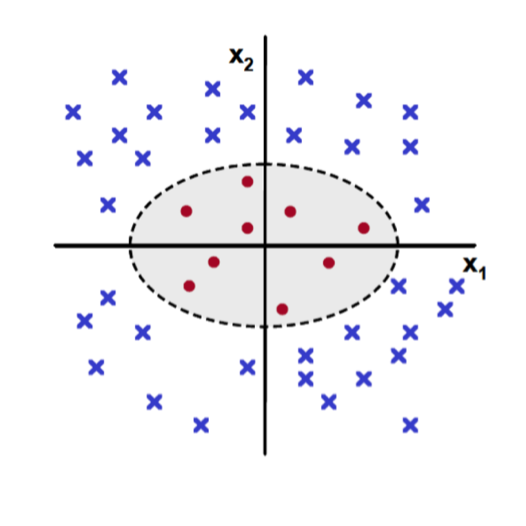
\includegraphics[width=.25\textheight,height =0.4\textheight]{figures/nonlinear2sets.png}} \xrightarrow[\text{feature map}]{\varphi(x,y) = x_1^2 + x_2^2} 
 	 \adjustbox{valign=c}{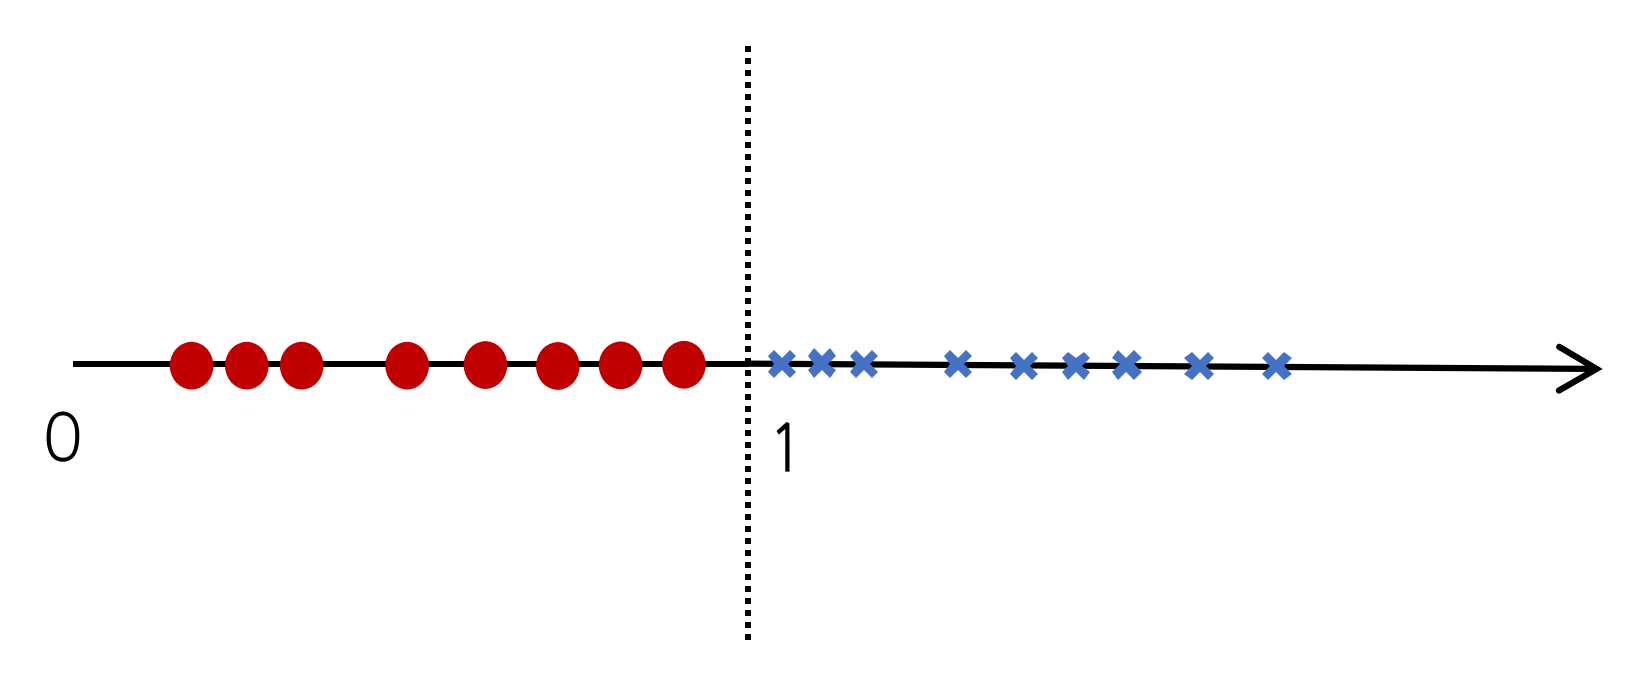
\includegraphics[width=.25\textheight]{figures/nonlinear2sets1D.png}}
 	 \end{equation*}
 \end{example}



Here we have the following comparison between linear and nonlinear models from the viewpoint of
loss functions:

\begin{description}
\item[Linear case (Logistic regression):] 
$$
L_{\lambda }(\theta) = \sum_{j=1}^N \ell (y_j, p(x_j; \theta)) + \lambda R(\|\theta\|),
$$
as defined in \eqref{eq:logisticlambda}.
\item[Nonlinear case: ]
$$
L_{\lambda }(\theta) = \sum_{j=1}^N \ell (y_j, p( \varphi(x_j; \theta_1); \theta_2)) + \lambda R(\|\theta\|).
$$
\end{description}
Here $p(x; \theta) = {\rm softmax}(Wx + b)$ where $\theta = (W,b)$,
and $\theta = (\theta_1, \theta_2)$ for the nonlinear case.
For both cases, $\displaystyle \ell(q, p) = \sum_{i=1}^k - q_i \log p_i$  represents the cross-entropy, and $\lambda R(\|\theta\|)$ is the  regularization term.
%\begin{remark}We have the following remarks.
%\begin{enumerate}
%	\item $\ell(q, p) = \sum_{i=1}^k - q_i \log p_i \leftrightarrow$  cross-entropy 
%	\item $p(x; \theta) = {\rm softmax}(Wx + b)$ where $\theta = (W,b)$
%	\item $\theta = (\theta_1, \theta_2)$ for nonlinear case
%	\item $\lambda R(\|\theta\|)$ $\leftrightarrow$  regularization term
%\end{enumerate}
%\end{remark}

In general, we have the following popular nonlinear models for $\varphi(x;\theta)$:
\begin{enumerate}
	\item Polynomials.
	\item Piecewise polynomials (finite element method).
	\item Kernel functions in SVM, see in Section \ref{sec:SVM}.
	\item Deep neural networks.
\end{enumerate}
 
 
 
 

\endinput

Based on the theorem of partition of unit, we may also have the next definition for 
nonlinear classifiable.
\begin{definition}[nonlinearly separable via partition of unit]
	These data sets $A_1, A_2, \cdots, A_k \subset \mathbb{R}^d$ are called nonlinearly separable, 
	if there exist smooth
	\begin{equation}\label{key}
	\varphi_i: \mathbb{R}^d \mapsto [0, 1], \quad i = 1, 2, \cdots, k,
	\end{equation}
	such that
	\begin{equation}\label{key}
	\varphi_i(x) = 1, x \in A_i  \text{ and } \varphi_i(0) = 1, x \in A_j,    \text{ for } i, j= 1, 2, \cdots, k \text{ but } j \neq i,
	\end{equation}
	and 
	\begin{equation}\label{key}
	\sum_{i=1}^k \varphi_i(x) = 1, \quad \forall x \in \mathbb{R}^d.
	\end{equation}
	are linearly separable.
\end{definition}

\begin{remark}
	For these next observations for definition of nonlinear separable via partition of unit.
	\begin{enumerate}
		\item Nonlinearly separable via partition of unit is a special case of nonlinear separable via feature mapping as
		we can always choose $\tilde d = k$ and
		\begin{equation}\label{key}
		\varphi(x) = \begin{pmatrix}
		\varphi_1(x) \\
		\varphi_2(x) \\
		\vdots \\
		\varphi_k(x)
		\end{pmatrix}.
		\end{equation}
		Then it is easy to verify that $\{\varphi(A_i)\}_{i=1}^k$ are linearly separable.
		\item Based on the properties of partition of unit, we can prove that if $A_i$ are
		finite sets, then there must exist the partition of unit which makes them must be nonlinearly separable.
%		\item 
	\end{enumerate}
\end{remark}

\subsection{Decision boundary}